
\chapter{Summary of FCS-Simulation in \df}
\label{sec:SummaryOfDf}
\label{sec:IntroductionToDf}
\section{Stepes of an FCS-Simulation}
\label{sec:StepesOfAnFCSSimulation}

The software \df was designed simulate FCS and FCCS correlation curves for different focus geometries and is closely related to the FCS/FCCS theory as presented in  chapter~\ref{sec:IntroductionToFCS} and Ref.~\cite{KRIEGERPHD2014} and especially the modeling of fluorescence detection described in section~\ref{sec:FCSModelingTheOpticalSystem}. It starts from a set of $N$ particle trajectories $\{\vr_i(t)\}$, where $i$ numbers the particles and $t=1,2,...$ numbers the equidistant timepoints with resolution $\Delta t_\txt{im}$. The trajectories are either read from an external data file or are created internally by a configurable random walk. First $N_i\geq 1$ fluorophores are assigned to each particle, leading to an overall number of fluorophores \[  F=\sum\limits_{i=1}^NN_i  \] fluorophores $f$, which are each  characterized by the following set of properties (the functions $i(f)$ is the trajectory ID for every fluorophore $f$):
\begin{enumerate}
	\item a position $\vr_f(t)=\vr_{i(f)}(t)+\Delta\vr_{f}$, where $\vr_{i(f)}(t)$ is the position of the particle and $\Delta\vr_f$ is an arbitrary, but constant shift from this position. In the simplest case there is only one fluorophore per particle and $\Delta\vr_f=0$. Using $\Delta\vr_f\neq0$, moving finite-sized objects may be simulated that are e.g. labeled with a set of fluorophores on their surface or in their interior.
  \item each fluorophore may be in one of $S_f$ states. Each state may have different spectroscopic properties. The current state at time $t$ is denoted by $s_f(t)$. 
  \item a wavelength-dependent absorption crosssection spectrum $\sigmaabsm{i}(\lambda)$.
  \item a normalized fluorescence spectrum $\eta_{\txt{fl},f}(\lambda)$ and a fluorescence quantum yield $\qfluorm{f,s_f(t)}$
  \item a dipole orientation vector $\vp_f(t)$ with $\snorm{\vp_f(t)}=1$.
\end{enumerate}
The state trajectory $s_f(t)$ for each fluorophore either does not change (the default case), is read from an external file, or is simulated using a matrix of transition rates and a random decision in each simulation step. In this way photophysical blinking transitions may be simulated, if e.g. $s_f(t)\equiv1$ is a bright state and $s_f(t)\equiv2$ is a dark state with $\qfluorm{f,2}=0$. Also a simple bleaching process is implemented, by switching off (but never on again) a fluorophore with a certain low probability.

The simulation proceeds in steps of $\Delta t_\txt{sim}$. For each time step and each focus in the simulation, first the expected number of fluorescence photons is calculated:
\begin{equation}\label{eq:app_sim_fcs_nphoton}
  \overline{N}_\txt{phot}(t)=\sum\limits_{f=1}^F\qfluorm{f,s_f(t)}\cdot\sigmaabsm{i}(\lambda_\txt{ex})\cdot q_\txt{det}\cdot \frac{\Delta t_\txt{sim}\cdot I(\vr_f(t))}{h\clight/\lambda_\txt{ex}}\cdot \Omega(\vr_f(t))\cdot h_\txt{pol}(\vp_f(t)),
\end{equation}
where $h$ is Planck's constant, $\clight$ is the velocity of light in vacuum and $\lambda_\txt{ex}$ is the excitation wavelength. 

The shape of the illumination profile is described by the function $I(\vr)$ and the respective shape of photon collection efficiency by $\Omega(\vr)$. Several models are implemented for them:
\begin{enumerate}
	\item \textbf{Gaussian}: The shapes of $I(\vr)$ and $\Omega(\vr)$ are cigar-like Gaussian functions with equal $x$- and $y$-width $w_0$ and $z$-width $z_0$:
					\begin{equation}\label{eq:sim3} I(\vr),\Omega(\vr)\propto\exp\left(-2\cdot\frac{x^2+y^2}{w_0^2}-2\cdot\frac{z^2}{z_0^2}\right) \end{equation}
	\item \textbf{Gaussian beam}: The illumination/detection focus is described by a Gaussian beam, which has a lateral width $w(z)$ increasing with distance $z$ from the focus and a Laurentzian shape in $z$-direction:  
					\begin{equation}\label{eq:sim4} I(\vr),\Omega(\vr)\propto\left(\frac{w_0}{w(z)}\right)^2\cdot\exp\left(-2\cdot\frac{x^2+y^2}{w^2(z)}\right),\ \ \ \ \text{with}\ \ \ w(z)=w_0\cdot\sqrt{1+\left(\frac{z}{z_0}\right)^2} \end{equation}
	\item \textbf{Gaussian light sheet}: A simple model for a lightsheet is a Gaussian in $z$-direction, which does not depend on $x$ or $y$:
					\begin{equation}\label{eq:sim5} I(\vr)\propto\exp\left(-2\cdot\frac{z^2}{z_0^2}\right) \end{equation}
	\item \textbf{Slit pattern light sheet}: To model the sidelobes observed in typical light sheets a slit function can be used:
					\begin{equation}\label{eq:sim6} I(\vr)\propto\left(\frac{\sin(\pi\cdot z/z_0)}{\pi\cdot z/z_0}\right)^2 \end{equation}
\end{enumerate}
The first two patterns can be used for both, the illumination and detection foci, whereas the last two are designed to model the light sheet illumination.

The remaining influence of the detection process (signal loss at optical interfaces and filters, detector quantum efficiency, ...) is described by the factor
\begin{equation}\label{eq:app_sim_fcs_qdet}
  q_\txt{det}=q_{\txt{det},0}\cdot\frac{\int\limits_{\lambda_\txt{det,min}}^{\lambda_\txt{det,max}}\eta_{\txt{fl},f}(\lambda)\;\dd\lambda}{\int\limits_{0}^{\infty}\eta_{\txt{fl},f}(\lambda)\;\dd\lambda},
\end{equation}
summarizing the loss of light due to optics and detector quantum efficiency $q_{\txt{det},0}$, as well as the spectral width of the fluorescence detection window $\lambda_\txt{det,min}...\lambda_\txt{det,max}$. This detection window allows to also take into account crosstalk between two detection channels. The influence of the dipole direction $\vp_f(t)$ and a possible laser polarization is modeled by the factor
\begin{equation}\label{eq:app_sim_fcs_hpol}
  h_\txt{pol}(\vp_f(t))=(1-\theta_\txt{pol})+\theta_\txt{Pol}\cdot\left(\vec{\epsilon}_\txt{ex}\bullet\vp_f(t)\right)^2,
\end{equation}
where $\bullet$ is a scalar product, $\theta_\txt{Pol}\in[0,1]$ is the fraction of linear polarization of the excitation light source and $\vec{\epsilon}_\txt{ex}$ (with $\snorm{\vec{\epsilon}_\txt{ex}}=1$) is the linear polarization direction of this light source.

From the average number of detected photons, the measured number of photons ${N}_\txt{det}(t)$ is calculated, taking the detector statistics into account. In the simplest case of a photon counting detector, ${N}_\txt{det}(t)$ is drawn from a Poissonian distribution with mean (and variance) $\overline{N}_\txt{phot}(t)$. Other detection statistics are possible, such as a linear detector, where ${N}_\txt{det}(t)$ is drawn from a Gaussian distribution with mean $\avg{G}\cdot\overline{N}_\txt{phot}(t)$ and a variance:
\begin{equation}\label{eq:app_sim_fcs_lindetnoise}
  \sigma_\txt{det}^2=\avg{G}^2\cdot\excessnoise\cdot{N}_\txt{det}(t)+\sigmaread^2,
\end{equation}
where $\avg{G}$ is the average detector gain, $\excessnoise$ the excess noise factor and $\sigmaread^2$ the read noise variance, summarizing all contributions, not depending on the number of incident photons. Also artifacts, such as a background intensity offset may be included in the detector simulation. Although intermediate results may be floating-point numbers, the finally detected number of photons (or ADU counts in a linear detector) is always an integer number.

Finally the time series  ${N}_\txt{det}(t)$ is post processed to yield count rate traces with arbitrary binning, auto- and cross-correlation functions (between different foci on the simulation) and other statistical properties. Also several test data sets are saved by the simulation program, such as particle \index{mean squared displacement}mean squared displacements (\index{MSD}MSDs), the raw detector statistics etc.

The complete program is split into modules that may be combined in different ways for a simulation. All these modules are either trajectory sources or sinks. In each time step first all sources generate a new set of fluorophore properties, e.g. by reading a new data set from a file or advancing a random walk simulation. The these new particle properties are forwarded to the sink objects, which simulate the actual detection process, as described above, or generate MSDs and other trajectory statistics. Every sink may be connected to several sources, and one source can feed several sinks. This can be used e.g. for simulations of fluorophore reservoir depletion, where a single trajectory source is fed into intermediate objects that simulate different bleaching rates on the same particle positions and finally detected by a set of identical sinks, which simulate FCS detection.

This software was developed during my PhD thesis. It has already been used to simulate different aspects of FCS/FCCS for several publications \cite{WOCJAN2009,BUCHHO2012,SINGHKRIEGER2013,KRIEGE2014}.



\section{Organization of \df}
\label{sec:OrganizationOfDf}
The software \df has been designed to mainly follow the steps, presented in the last section, but in a very configurable way. The simulation is set up, as a combination of two classes of objects:
\begin{itemize}
	\item \textbf{(fluorophore) dynamics objects}\index{fluorophore dynamics}\index{generator object}\index{trajectory generator}\index{trajectory source} that simulate the motion of detectable particles. Each such object outputs a list of the positions and properties of all the particles it simulates. These properties may be generated by a dynamic simulation, or they can be read from external data-files (e.g. the output of another simulation software, as described in \cite{WOCJAN2009}). It is even possible to base the output of a trajectory generator object on the trajectories from another object, e.g. adding a fluorophore of a second color to a particle. 
	\item \textbf{(fluorescence) detection objects}\index{detection object}\index{fluorescence detection object}\index{trajectory sink} that accept the trajectories as input and generate some kind of output from them (e.g. FCS correlation curves from the fluorescence in a virtual microscope focus, MSD-curves, ...).
\end{itemize}
Of both classes, several different object types exist. They are listed and explained in more detail in chapter~\ref{sec:ReferenceOfTheDfModules}. You can even write your own new classes using C++ and use them in a simulation. This is explained in chapter~\ref{sec:ReferenceOfTheDfModules}. Then the simulation is set up by instantiating at least one trajectory generator and at least one detection object and connecting them in an appropriate way. The setup of a simuation is denoted in a \itindex{configuration file} (often also called \itindex{INI-file}). The next section~\ref{sec:AMinimalExample} will introduce these concepts with a simple (and basic) example.

\section{A Minimal Example}
\label{sec:AMinimalExample}
A very simple configuration for \df could look as follows:
\begin{lstlisting}[language=INI] 
##################################################################
# simulation setup
##################################################################
simulation.duration=0.1     # duration of the simulation in seconds
simulation.timestep=1e-6    # simulation timestep in seconds
# prefix for all output files 
#    tosystempathseparator() converts \ and / to your locally
#    valid filename separator
simulation.basename=tosystempathseparator("./diffusion4_test/")

##################################################################
# setup all brownian objects ("supergroup")
##################################################################
brownian.volume_shape=sphere             # spherical volume 
brownian.sim_radius=3                    # with 3 micrometer radius
brownian.init_fluorophor=atto488         # fluorophore is al488


##################################################################
# setup all fcs objects ("supergroup")
##################################################################
# resolution of the "FCS-data acquisition"/minimum lag-time [seconds]
fcs.corr_taumin=simulation.timestep*2
fcs.corr_S=20              # number of blocks in correlator
                           # taumax ~ corr_taumin*8*2^S
fcs.P0=150                 # laser power in microWatt above objective
fcs.lambda_ex=488          # excitation laser wavelength in nanometers
fcs.expsf_r0=0.33          # 1/e^2 width of excitation volume [micrometers]
fcs.expsf_z0=6*0.33        # 1/e^2 width of excitation volume [micrometers]
fcs.detpsf_r0=fcs.expsf_r0 # detection volume size = excitation volume size
fcs.detpsf_z0=fcs.expsf_z0
fcs.q_det=1                # detection efficiency
fcs.save_binning=true      # save binned countrate
fcs.save_binning_time=0.005# 5ms binning


##################################################################
# dynamics object "brownian1"
##################################################################
brownian1.diff_coeff=50    # diffusion coefficient [micron^2/sec]
brownian1.c_fluor=10       # concentration [nM]


##################################################################
# detection object "fcs1"
##################################################################
fcs1.sources=brownian1       # get trajectories from brownian1
fcs1.object_name=particlesA  # a custom name for the fcs1-object
\end{lstlisting}

\noindent As you can see, the configuration has a simple structure:
\begin{itemize}
  \item comments are started with the character ``\texttt{\#}'' and stop at the end of the line
	\item each line is an assignment to a property:
		\begin{center}
			\texttt{property\_group.property\_name = }	\textit{value}
		\end{center}
	\item Each property belongs to a group of properties, such as:
	\begin{itemize}
		\item \texttt{simulation}: basic simulation settings, such as the duration, or timestep
		\item \texttt{fcs}: presets for all ``fcs'' detection-objects in the simulation
		\item \texttt{brownian}: presets for all ``brownian'' dynamics-objects in the simulation
		\item \texttt{fcs1}: properties of the concrete detection-object ``fcs1'' (to instantiate a detection object, you have to set at least one of its properties!)
		\item \texttt{brownian1}: properties of the concrete dynamics-object ``brownian1'' (to instantiate a dynamics object, you have to set at least one of its properties!)
	\end{itemize}
	\item as \textit{value} you can either give numbers (``.'' as decimal separator), simple strings (potentially in double-quotes), or a boolean value \texttt{true} or \texttt{false}.
	\item In addition it is possible to denote simple mathematical expressions as \textit{value}. In these you can calculate with the three basic datatypes number, string and boolean. All properties that have already been defined in the file can be used. Here is an example from the file:
	\begin{center}
		\texttt{fcs.corr\_taumin = simulation.timestep*2}
	\end{center}
	This sets \texttt{fcs.corr\_taumin} to 2-times the simulation timestep \texttt{simulation.timestep}. In these expression, you can use the standard C-functions, like \texttt{sin(), cos(), exp(), sqrt(), pow(), ...} and several special functions like \texttt{floattostr(), booltostr(), if()}. Strings can be concatenated with the operator \texttt{+}.
\end{itemize}


The  configuration script, given above, will run a simulation of one species of particles (\texttt{brownian1}) with a diffusion coefficient of $50\unit{\mu m^2/s}$ and at a concentration of $10\unit{nM}$. An Alexa-488-fluorophore (\texttt{al488}) is attached to each particle and they are excited by a laser at $488\unit{nm}$, which forms a virtual Gaussian focus with a $1/\ee^2$-halfwidth of $w_\txt{xy,ex}=0.33\unit{\mu m}$ and a $1/\ee^2$-halflength of $w_\txt{z,ex}=6\cdot0.33\unit{\mu m}\approx2\unit{\mu m}$. A detection focus with the same position and sizes ($w_\txt{xy,det}=w_\txt{xy,ex}$,$w_\txt{z,det}=w_\txt{z,ex}$) is used to detect the photons. therefore the effective focus used in the FCS-equations will have a size of:
  \[ w_\txt{xy}=\sqrt{\frac{1}{1/w_\txt{xy,det}^2+1/w_\txt{xy,ex}^2}}\approx0.23\unit{\mu m},\ \ \ \ \ w_\txt{z}=\sqrt{\frac{1}{1/w_\txt{z,det}^2+1/w_\txt{z,ex}^2}}\approx1.38\unit{\mu m} \]
The simulation runs for $0.1\unit{s}$ with a timestep of $\Delta t_\txt{sim}=1\unit{\mu s}$. The minimum lag-time of the correlator is set to $\tau_\txt{min}=2\cdot\Delta t_\txt{sim}$. Finally, the correlator has $S=20$ linear correlator blocks, which amounts to a maximum lag-time of approximately:
  \[ \tau_\txt{max}\approx m^S\cdot P/2\cdot\tau_\txt{min}\approx17\unit{s}\ \ \ \ \ \left[\text{default:}\ \ m=2, P=16\right] \]
The configuration of the simulation can be drawn as a simple diagram, as shown in \figref{fig:simplexample_struc}
The resulting correlation curves will look approximately like the one shown in \figref{fig:simplexample}.

The simulation outputs its results into files that are composed of:
\begin{center}
	\texttt{simulation.basename} + \textit{object-name} + \textbf{\textit{description}.\textit{extension}}
\end{center}
In the file above, the \texttt{simulation.basename} will be \texttt{./diffusion4\_test/}, which indicates a sub-directory  ``diffusion4\_test'' in the execution directory of \df. The \textit{object-name} can either be ``brownian1'' for output by the dynamics object, or ``particlesA'' for output from the detection object fcs1 (it would be ``fcs1'', if \texttt{fcs1.object\_name} wouldn't have been given). Note that the \textit{object-name} is optional and there will also be some output files with only \textit{description}.\textit{extension}, e.g. the files \texttt{config.txt} and \texttt{log.txt}, which contain general log-output and properties of the simulation. There is also a file \texttt{config.gv}, which can be interpreted by \textsc{GraphViz} (see section~\ref{sec:UsefullAdditionalTools}) to draw the structure in \figref{fig:simplexample_struc}. Finally the file \texttt{config.ini} contains an extended copy of the simulation configuration files.


\begin{figure}[t!]
	\centering
		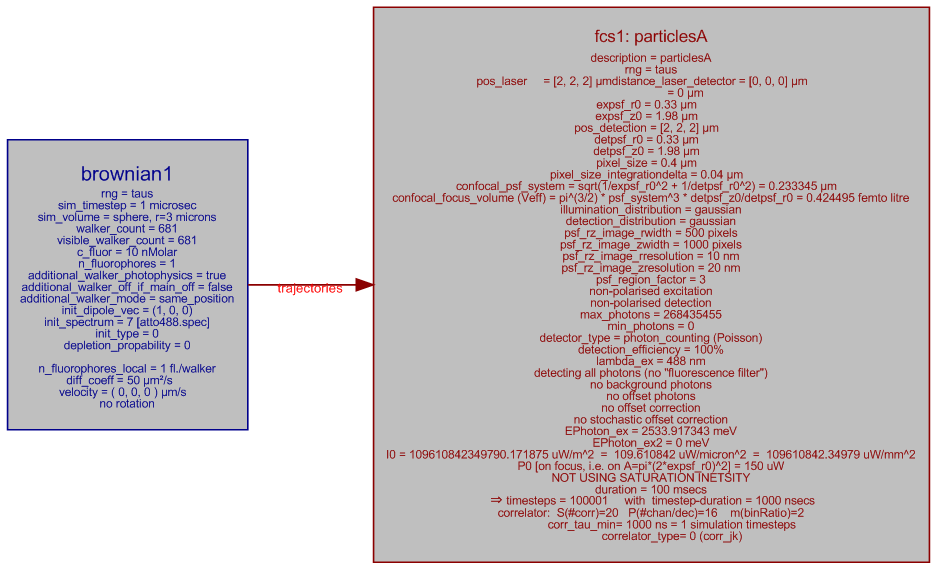
\includegraphics[width=0.9\textwidth]{pic/simplexample_struc.png}
	\caption{Project structure of the simple example}
	\label{fig:simplexample_struc}
\end{figure}
\begin{figure}[b!]
	\centering
		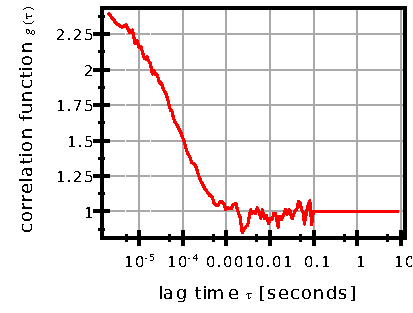
\includegraphics{pic/simplexample.pdf}
		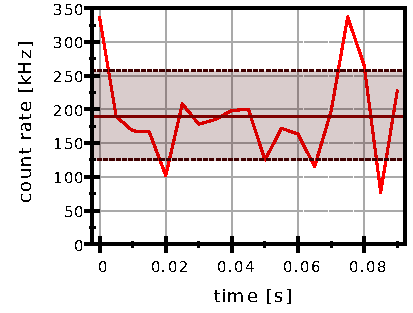
\includegraphics{pic/simplexample_cnt.pdf}
	\caption{Correlation and countrate curves from the simple example script}
	\label{fig:simplexample}
\end{figure}

The output-files from brownian1 and fcs1 contain different checks of the simulation software and also different types of additional outputs. The majow files from fcs1/particlesA are:
\begin{itemize}
	\item \texttt{particlesA\textbf{alvacf.asc}}, \texttt{particlesA\textbf{.qf3acorr}}\\ output correlation curves (together with countrate traces) either in the ALV-5000 ASCII-format, or in a generic ASCII-format that is understood by \qf
	\item \texttt{particlesA\textbf{bts.dat}}, \texttt{particlesA\textbf{btsplot.plt}}\\ countrate-trace as CSV-file and a \textsc{GnuPlot}-script to plot it
	\item \texttt{particlesA\textbf{corr.dat}}, \texttt{particlesA\textbf{corrplot.plt}}\\correlation curve as CSV-file and a \textsc{GnuPlot}-script to plot it
	\item \texttt{particlesA\textbf{detbackgroundtest.plt}}\\\textsc{GnuPlot}-file with different checks of the background countrate in the detector of the FCS-simulation
	\item \texttt{particlesA\textbf{dettest.plt}}\\\textsc{GnuPlot}-file with different checks of the detector statistics of the FCS-simulation
	\item \texttt{particlesA\textbf{psf.plt}}\\\textsc{GnuPlot}-file with different characteristics of the excitation and detection focus of the FCS-simulation
\end{itemize}

\section{A Simple 2-Component Diffusion Simulation}
\label{sec:ASImple2ComponentDiffusionSimulation}
Starting from the simple example in the last section, we can extend it to show more features of \df. First we will do a 2-component diffusion simulation with two types of walkers with different diffusion coefficients. To do so, we will instantiate two instead of one \texttt{brownian} objects (the rest of the simple script stays un-altered, except potentially \texttt{simulation.duration=0.5}):
\begin{lstlisting}[language=INI] 
##################################################################
# dynamics object "brownian1"
##################################################################
brownian1.diff_coeff=100   # diffusion coefficient [micron^2/sec]
brownian1.c_fluor=2        # concentration [nM]

##################################################################
# dynamics object "brownian2"
##################################################################
brownian2.diff_coeff=1    # diffusion coefficient [micron^2/sec]
brownian2.c_fluor=2       # concentration [nM]
\end{lstlisting}
Now we have two populations of (independently) diffusiong particles: fast ones ($D=100\unit{\mu m^2/s}$) in \texttt{brownian1} and slow ones ($D=1\unit{\mu m^2/s}$) in \texttt{brownian2}. For both of them, the same abundance of $c=2\unit{nM}$ was set.
For the detection we again use a single \texttt{fcs}-object, but now it takes the trajectories from two sources:
\begin{lstlisting}[language=INI] 
##################################################################
# detection object "fcs1"
##################################################################
fcs1.sources=brownian1,brownian2 # get trajectories from brownian1
                                 # and brownian2
\end{lstlisting}
This constructs a project with a structure as shown in \figref{fig:simple2comp_struct}.
The results of such a simulation (also in comparison to a simple 1-component simulation with $D=100\unit{\mu m^2/s}, c=4\unit{nM}$ is shown in \figref{fig:simple2comp_acf}.

\begin{figure}[b!]
	\centering
		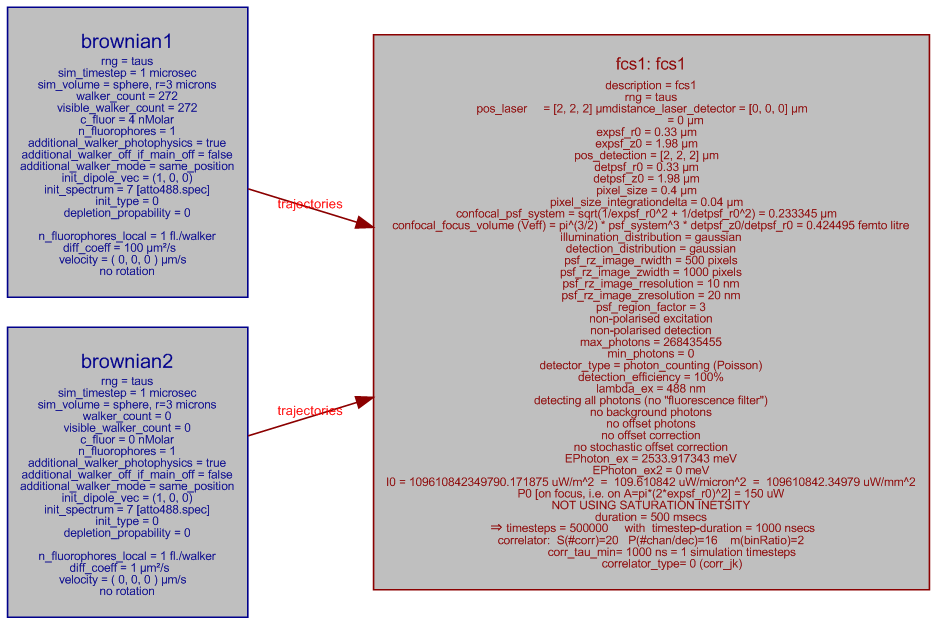
\includegraphics[width=0.9\textwidth]{pic/simple2comp_struct.png}
	\caption{Structure of a 2-component diffusion configuration}
	\label{fig:simple2comp_struct}
\end{figure}



\begin{figure}[t!]
	\centering
		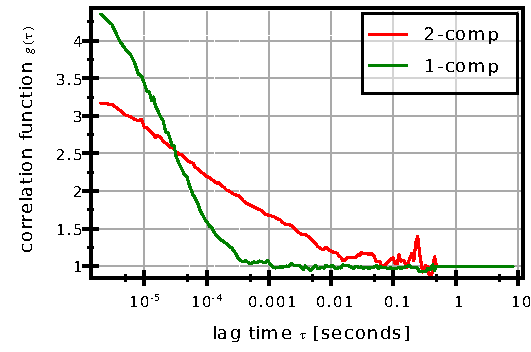
\includegraphics{pic/simple2comp_acf.pdf}
	\caption{Results from a 2-component simulation}
	\label{fig:simple2comp_acf}
\end{figure}
